
\documentclass{llncs}

\usepackage{url}
\usepackage{graphics}

\newcommand{\workingnote}[1]{}        % The version that hides the note.
%\newcommand{\workingnote}[1]{(**#1)}   % The version that makes the note visible.

\renewcommand\url{\begingroup \def\UrlLeft{<}\def\UrlRight{>}\urlstyle{tt}\Url}
\newcommand\emailaddr{\begingroup \def\UrlLeft{<}\def\UrlRight{>}\urlstyle{tt}\Url}
% REMIND: there's a bug in the URL package that puts '%' in the second line
% of a wrapped URL.

%\newif\ifpdf
%\ifx\pdfoutput\undefined
%   \pdffalse
%\else
%   \pdfoutput=1
%   \pdftrue
%\fi

\begin{document}

%% Use dvipdfm instead. --DH
%\ifpdf
%  \pdfcompresslevel=9
%  \pdfpagewidth=\the\paperwidth
%  \pdfpageheight=\the\paperheight
%\fi

\title{Mixminion: Type III Anonymous Remailer Design}
\author{George Danezis\inst{1} \and Roger Dingledine\inst{2} \and David Hopwood\inst{3}
        \and Nick Mathewson\inst{2}}
\institute{Cambridge
\email{\emailaddr{george.danezis@cambridge}}
\and
The Free Haven Project
\email{\emailaddr{arma@mit.edu}}
\and
Independent consultant
\email{\emailaddr{david.hopwood@zetnet.co.uk}}
}
\maketitle
\pagestyle{empty} 
  
\begin{abstract}

We describe a packet-based anonymous remailer protocol that supports
secure single-use reply blocks and includes link-level encryption to provide
forward anonymity. We describe designs for directory servers and nymservers,
and discuss their anonymity implications.
% We include justification
%for various design decisions and a detailed description of attacks and
%defenses. And some other stuff.

\end{abstract}

\textbf{Keywords:} anonymity, MIX-net, peer-to-peer, remailer, nymserver, reply block %, ...

%%%%%%%%%%%%%%%%%%%%%%%%%%%%%%%%%%%%%%%%%%%%%%%%%%%%%%%%%%%%%%%%%%%%%%%

\section{Introduction}
\label{sec:intro}

Chaum first introduced anonymous remailer designs over 20 years ago
\cite{chaum-mix}. The research community has since introduced many new
designs and proofs \cite{big-chain-of-cites}, and discovered a variety
of new attacks \cite{more-cites}, but the
state of deployed remailers has changed remarkably little since Cottrell
published his Mixmaster software \cite{mixmaster-attacks} in 1994. 
Part of the difficulty in expanding the deployed remailer base is
due to the liability involved in running a remailer node on the Internet,
and part is due to the complexity of the current infrastructure ---
it is very hard to add new experimental features to the current software.

The Mixminion project aims to deploy a cleaner updated remailer design
in the same spirit as Mixmaster, with the goals of expanding deployment,
documenting our design decisions and how well they stand up to all known
attacks, and providing a research base for experimental features. We
describe our overall design in Section \ref{sec:design}, including
a new primitive called a \emph{single-use reply block}
(SURB).  Mixmaster provides no support for replies, instead relying
on the older and less secure cypherpunk Type I remailer design
\cite{remailer-history}. By integrating reply capabilities into
Mixminion, we can finally retire the Type I remailer network.

We introduce link-level encryption with ephemeral keys to ensure forward
anonymity for each message. We also provide flexible delivery schemes ---
rather than just allowing delivery to mail or Usenet, we allow designers
to add arbitrary modules to handle incoming and outgoing messages. By
separating the core mixing architecture from these higher-level modules,
we can limit their influence on the anonymity properties of the system. We
go on in Section \ref{sec:dir-servers} to describe a design for directory
servers to track and distribute remailer availability, performance,
and key information, and then describe in Section \ref{sec:nymservers}
how to securely build higher-level systems such as nymservers using SURBs.

Mixminion aims to be a best-of-breed remailer that uses conservative
design approaches to provide security against most known attacks.
Many of our design decisions impact anonymity in surprising ways. Herein
we document and analyze some of these influences to provide more intuition
to developers and users.

%%%%%%%%%%%%%%%%%%%%%%%%%%%%%%%%%%%%%%%%%%%%%%%%%%%%%%%%%%%%%%%%%%%%%%%

\section{Related Work}

\subsection{MIX-nets}

Chaum introduced the concept of a MIX-net for anonymous communications
\cite{chaum-mix}. A MIX-net consists of a group of servers, called MIXes
(or MIX nodes), each of which is associated with a public key. Each
MIX receives encrypted messages, which are then decrypted, batched,
reordered, and forwarded on without any information identifying the
sender. Chaum also proved security of MIXes against a \emph{passive
adversary} who can eavesdrop on all communications between MIXes but is
unable to observe the reordering inside each MIX.

Current research directions on MIX-nets include ``stop-and-go'' MIX-nets
\cite{kesdogan}, distributed ``flash MIXes'' \cite{flash-mix} and their
weaknesses \cite{desmedt,mitkuro}, and hybrid MIXes \cite{hybrid-mix}.

One type of MIX hierarchy is a cascade.
In a cascade network, users choose from a set of fixed paths through
the MIX-net. Cascades can provide greater anonymity against a large
adversary, because in a free-route system an
adversary who owns many of the MIXes can use intersection attacks to
dramatically reduce the set of possible senders or receivers for a given
message \cite{disad-free-routes}.
MIX cascade research includes real-time MIXes \cite{realtime-mix} and
web MIXes \cite{web-mix}.

\subsection{Deployed Remailer Systems}

The first widespread public implementations of MIXes were produced by the
cypherpunks mailing list. These ``Type I'' \emph{anonymous remailers}
were inspired both by the problems surrounding the {\tt anon.penet.fi}
service \cite{helsingius}, and by theoretical work on MIXes. Hughes wrote
the first cypherpunks anonymous remailer \cite{remailer-history}; Finney
followed closely with a collection of scripts which used Phil Zimmermann's
PGP to encrypt and decrypt remailed messages. Later, Cottrell implemented
the Mixmaster system \cite{mixmaster}, or ``Type II'' remailers, which
added message padding, message pools, and other MIX features lacking
in the cypherpunk remailers. At about the same time, Gulcu and Tsudik
introduced the Babel system \cite{babel}, which also created a practical
remailer design (although one that never saw widespread use).

\subsection{Robustness}

Some previous work investigates a notion of the \emph{robustness}
of MIX-nets in the context of a distributed MIX system
\cite{flash-mix}. A MIX is considered robust if it survives the
failure of any $k$ of $n$ participating servers, for some threshold
$k$. This robustness is all or nothing: either $k$ servers are
good and the MIX works, or they are not good and the MIX likely will
not work.

Robustness has been achieved primarily via the use of zero-knowledge
proofs of correct computation; participants use such proofs to convince
each other that they follow the protocol correctly without revealing secret
information. Done na\"{\a i}vely, this incurs significant
overhead. 
Jakobsson showed how to use precomputation to reduce the overhead of
such a MIX network to about 160 modular multiplications
per message per server \cite{flash-mix}, but the protocol was later
found to be flawed \cite{mitkuro} by Mitsumo and Kurosawa. They
proposed a fix for the protocol, but the efficacy of this fix remains
to be evaluated.  A different approach was taken by Desmedt and
Kurosawa \cite{desmedt}, but their technique requires many
participating servers. Other work, such as Abe's MIX \cite{abe},
provides \emph{universal verifiability} in which any observer can
determine after the fact whether a MIX cheated or not, but
the protocol is still computationally expensive.

\subsection{Remailer Statistics}

Levien's \emph{statistics pages} \cite{levien} track both remailer
capabilities (such as what kinds of encryption the remailer supports)
and remailer up-times, observed by pinging the machines in question
and by sending test messages through each machine or group of machines.
Such \emph{reputation systems} improve the reliability of MIX-nets by
allowing users to avoid choosing unreliable MIXes. The Jack B Nymble 2
remailer client \cite{potato} allows users to import statistics files
and can then pick remailers according to that data. Users can specify
minimum reliability scores, decide that a remailer should always or never
be used, and specify maximum latency. Ongoing research on more powerful
reputation systems includes a reputation system for free-route networks
\cite{mix-acc} and another for MIX cascades \cite{casc-rep}.

%%%%%%%%%%%%%%%%%%%%%%%%%%%%%%%%%%%%%%%%%%%%%%%%%%%%%%%%%%%%%%%%%%%%%%%

\section{A MIX-net with Secure Replies}
\label{sec:design}

Mixminion aims to bring together the current best approaches for providing
anonymity in a batching message-based MIX environment. We don't aim
to provide low-latency connection-oriented services like Freedom
\cite{freedom} or Onion Routing \cite{goldschlag99} --- while those
designs are more effective for common activities like anonymous web
browsing, it seems they cannot yet provide the same level of strong
anonymity as slower message-based services. Indeed, we intentionally
further restrict the set of options for users: we provide only one
cipher, and we avoid extensions that would help an adversary divide the
anonymity set.

Mixminion uses the same general MIX-net paradigm as previous work
\cite{chaum-mix, mixmaster-attacks, others}. The sender Alice chooses
a path through the network.
% consisting of $k$ MIXes, $N_1 \dots N_k$.
She repeatedly ``onion'' encrypts her message, starting with the last
MIX in her path, and sends the onion to the first MIX in her path. That
MIX processes the onion and passes the unwrapped-by-one-layer onion to
the next MIX, and so on. We describe the behavior of the last MIX in
Section \ref{subsec:delivery-modules}.

While Mixminion protects against known \emph{traffic analysis} attacks
(where an adversary attempts to link a given message to its sender or
receiver \cite{jfraymond, simon}), we do not fully address \emph{traffic
confirmation} attacks. In a traffic confirmation attack, the adversary
treats the MIX network as a black box and observes the behavior of
senders and receivers. Over time, he can intersect the set of senders
and receivers who are on-line at certain times and learn who is sending
and receiving which messages \cite{langos02}. Good dummy traffic designs
may eventually address the intersection attack, but for now it remains
an open problem.

We choose to drop backward-compatibility with Mixmaster and the cypherpunk
remailer systems, in order to provide a simple extensible design. At
the same time, we provide a new feature: a reply block mechanism that
is as secure as forward messages.

Reusable reply blocks are security risks --- by their very nature they
let people send multiple messages to them. These multiple messages can be
used to very quickly trace the recipient's path: if two incoming batches
both include a message to the same reply block, then the next hop must
be in the intersection of both outgoing batches.
Thus Mixminion uses single-use reply blocks to provide secure replies.

%%i will put this stuff later.
%Parties that benefit from anonymity properties must run dedicated software
%to be able to communicate with the remailer network; but other parties
%do not.
%Mixminion aims to minimize the traffic analysis value any compromised
%node could extract from passing messages. The protocol doesn't leak
%the position of the intermediary node in the chain or the total length
%of the route. Exceptions to this are exit nodes, where a route ends,
%and in the case of the ``swap headers'' method, described below, the
%the node that performs the crossover.

The rest of this section describes the motivation for secure replies,
including some new attacks and how we defeat them. We also discuss using
link-level encryption with ephemeral keys to provide forward anonymity,
message types and modules for handling different types of messages, and
exit policies for advertising what delivery options a node will provide.

%The rest of this section describes the header structure and the
%protocol for building and processing messages. In particular, we
%focus on two competing ways of providing secure reply functionality,
%and the tradeoffs and design decisions surrounding each approach. In
%the first approach, we provide a mechanism for implementing replies so
%that a reply message is indistinguishable from a forward message. Because this
%approach introduces some attacks that we cannot adequately address, we
%then propose a second approach that allows forward and reply messages
%to be distinguished but provides better overall security.


\subsection{Indistinguishable replies}
\label{subsec:header-swap}

Making forwards and replies indistinguishable prevents an adversary from
dividing the message anonymity sets into two classes. In particular, if
there are very few replies during a given period relative to the total
number of messages, an adversary controlling some of the MIXes in the
network can more easily trace the path of each reply --- even though
the batches may be large, the number of replies in each batch will be
quite small.

At the same time, protocols like Mixmaster include hashes of the entire
message in each header. Each hop in the path checks the integrity of
the header and payload, and drops the message immediately if it has been
altered. But since the author of the reply block is not the one writing
the payload, these hashes can no longer be used. Indeed, since we choose
to make forward messages and replies indistinguishable, we cannot provide
hashes for forward messages either. This choice introduces a new class
of attacks known as \emph{tagging attacks}.

\begin{figure}
\begin{center}
\resizebox{10cm}{!}{\includegraphics{SWAP.eps}}
\caption{The operations requered by the ``swap'' method} 
\end{center}
\end{figure}

A ``header swap'' mechanism could be used in order to minimize the
information leaked by \emph{tagging attacks}. Each mixminion packet,
when created, has two headers: the first one contains a series of sub
headers each encrypted as an onion under the public keys of a sequence of
nodes. Each of these sub headers contain some symmetric key and a hash
to check the integrity of the header. The second header contains sub
headers in the form of an onion as well but is also encrypted under
the keys contained in the first header, as well as the hash of the
payload. In the case of a bi-directional anonymous channel the 
second header could also be a single use reply block (SURB)
provided by another party. The payload is finally encrypted using all
the keys contained in the first header and the second if it is not a SURB.

The packet travels through nodes that perform the operations illustrated
on \emph{figure 1}. Each node decrypts the RSA sub header, retrieves
the key and checks the integrity of the first header. If someone has
tampered with it, the packet is discarded. If the header is correct,
the secret is used to decrypt the second header and the payload. There
is one special node, at the ``crossover point'', in the path that in
addition to the standard operation, decrypts the second header using
the hash of the payload and swaps the two headers.

The primitive used for encryption and decryption is BEAR \cite{BEAR},
a variable block size block cipher. It offers the property that if any
bit of the encrypted material is changed the decryption will look like
random bits for anyone that does not know the key. Therefore we minimize
an attackers benefit from tagging a message. It is impossible to tag the
headers because any modification is detectable. It is also fruitless to
modify the payload of the message: if it is modified before the crossover
point, the second header will not be decryptable, and if it is modified
afterward the first part of the path should offer enough anonymity. Of
course in order to make this scheme as secure as if tagging attacks did
not exist we should require users to choose the double path length for
each message. In practice users might choose to select shorter paths,
given that the remaining tagging attack provides very little information 
and is very difficult to mount.

\subsection{Approach two: the `distinguish replies' method}
\label{subsec:distinguish-replies}

%David? :)

\subsection{Link-level encryption and what it gets us}

Unlike remailer Types I and II that used SMTP as their underlying 
transport mechanism, Mixminion clients and nodes communicate using a
forward secure encrypted channel based on TLS \cite{TLS}.  TLS allows
the establishment of an encrypted tunnel using ephemeral
Diffie-Hellman keys. In order to make sure that the receiving end is
the one intended by the creator of the anonymous message, the
ephemeral key could be signed by the receiving node. As soon as a
session key has been established the Diffie-Hellman keys are destroyed
and messages start being sent through the tunnel. After each message a
standard key update operation is performed to generate a fresh key and
the old key material is deleted. Key updates don't use any asymmetric
encryption techniques, so they are fast.

The above scheme offers forward secrecy in the sense that after the keys
have been deleted even the
nodes that exchange messages are not able to decrypt or even recognize
messages that might have been intercepted on the links. This makes it
impossible to comply with decryption notices that might be served in
some jurisdiction.  It also makes it necessary for an adversary to
corrupt and control nodes in order to have enough information to trace
back a forward anonymous communication by requesting nodes to decrypt
it. (Reply blocks can still be used for this purpose.)  Even if an
attacker manages to get hold of the session key at a particular point
they would have to observe all subsequent traffic to be able to update
their key appropriately.

The forward secure encrypted channel offers only limited protection
against traffic analysis. Encrypted links between honest nodes prevent
an adversary from recognizing even his own messages; but without
link padding, he is still able to measure how much traffic is being
transmitted.

\subsection{Message types and delivery modules}
\label{subsec:delivery-modules}

Once a Mixminion packet reaches the final MIX in its path, it must be
dropped (if it is a dummy message), or delivered to its intended
recipient (if it is not).  In order to support different kinds of
delivery, each header contains a type code for the action to be taken
to deliver the message.  A few types--such as DUMMY, SMTP, and LOCAL
DELIVERY--are specified as a part of the Mixminion standard.  Others
may be added by future extensions, in order to implement
abuse-resistant exit policies (see Section \ref{subsec:exitpolicies}),
to administer nymservers (see Section \ref{sec:nymservers}), to publish
anonymously to Usenet, or to support other protocols.

% We never reached a consensus (afaik) on whether 'FORWARD' and 'DROP'
% were types or not.  Are they? -Nick

Nearly all delivery methods require additional information beyond the
message type and its payload.  The SMTP module, for example, requires
a mailbox name.\footnote{A {\it mailbox name} is the ``{\tt user@domain}''
part of an e-mail address. Mixminion uses only mailbox names in the
protocol, because the comment parts of an e-mail address could potentially
be different for senders who have obtained an address from different
sources, leading to a reduction in anonymity sets.}
In our current design, this information is placed
in a variable-length annex to the final header\footnote{It must be
in the header, since putting delivery information in the payload would
prevent people from creating SURBs that can be delivered by SMTP.
On the one hand, under the ``header swap'' method described in
\ref{subsec:header-swap}, the all-or-nothing property of BEAR prevents
the generator of a reply block from putting any information in the
payload.  On the other hand, under the ``distinguish replies'' method
in \ref{subsec:distinguish-replies}, the delivery information would
create a portion of the payload that the final node it could
distinguish from random garbage, thus allowing a tagging attack
against the reply block.}.
% See my messages of April 9 and 10 titled ``SMTP service'' for a more
% detailed version of the above argument. -Nick
%
% Should we say _why_ it's undesirable to force reply recipients to
% run local nodes?  [My answer is (A) that some people (such as human
% rights activists using internet cafes) want to get replies, but
% don't have persistant net connections, (B) that Mixmaster
% supports it, and not doing so would be a step backwards, and (C)    
% that there's not much reason not to.]    -Nick

The types each MIX supports are described in a \emph{capability
block}, which also includes the MIX's address, long-term (signing)
public key, short-term key (for use in header encryption), and
forwarding strategy (if any).  MIXes sign these capability blocks, and
publish them on directory servers (see section \ref{sec:dir-servers}).
Clients download this information from the directory servers.

% Is all of the stuff above really in the caps block?  Or do we break
% the volatile part (short-term key) from the nonvolatile part? -Nick
%
% I think they should be in the same block, although probably
% "capability block" isn't a good name for it. Capabilities should
% also be able to change without losing identity/reputation, and
% there would be no point in having two separate update mechanisms. --DH

The possibility of multiple delivery methods doesn't come free: their
presence may fragment the anonymity set.  For example, if there were 5
ways to send a SMTP message to Bob, an attacker could partition Bob's
incoming mail by assuming that one of those ways was Alice's favorite.
Furthermore, an active attacker Mallory could lure users into using an
exit node he had compromized by advertising that node as supporting a
rare but desirable delivery method.

We claim that these attacks do not provide an argument against
extensibility \emph{per se}, but rather argue against the proliferation
of redundant extensions, and against the use of rare extensions.  

\subsection{Exit policies and abuse}
\label{subsec:exitpolicies}

One important entry in a node's capability block is its \emph{exit
policy}. Exit abuse is a serious barrier to wide-scale remailer deployment
--- rare indeed is the network administrator tolerant of machines that
potentially deliver hate mail to the U.S. President.

On one end of the spectrum are \emph{open exit} nodes that will
deliver anywhere; on the other end are \emph{middle-man} nodes that
only relay traffic to other remailer nodes. More generally, nodes can
set individual exit policies to declare which traffic they will let
exit from them, such as traffic for local users or other authenticated
traffic \cite{onion-discex00}.

Preventing abuse of open exit nodes is an unsolved problem. If
receiving mail is opt-in, an abuser can forge an opt-in request from
his victim. Indeed, requiring recipients to declare their interest
in receiving anonymous mail is risky --- human rights activists in
Guatemala cannot both sign up to receive anonymous mail and also retain
plausible deniability.\footnote{
  Compare with the 1965 U.S. Supreme Court case Lamont v. Postmaster
  General (381 U.S. 301), where the Post Office would detain mail it
  deemed to be `communist political propaganda' and instead send a form
  to the addressee telling him to send back the signed form if he wanted
  to receive such mail. The government maintained a list of citizens
  who had filled out these forms.
}. Similarly, if receiving mail is opt-out, an abuser can deny service
by forging an opt-out request from a legitimate user. We might instead
keep the mail at the exit node and send a note to the recipient
telling them how to collect their mail; but this increases
server liability by storing messages (see Section \ref{sec:nymservers}
below), and also doesn't really solve the problem.

Of course, a mixture of open and restricted exit nodes will allow the
most flexibility for volunteers running servers. But while a large number
of middle-man nodes is useful to provide a large and robust network, the
small number of exit nodes still simplifies \emph{traffic confirmation}
(attacks where the adversary observes both a suspected user and the
network's exit nodes and looks for timing or packet correlations). The
number of available open exit nodes remains a limiting security parameter
for the remailer network.

%%%%%%%%%%%%%%%%%%%%%%%%%%%%%%%%%%%%%%%%%%%%%%%%%%%%%%%%%%%%%%%%%%%%%%%

\section{Directory Servers}
\label{sec:dir-servers}

The Mixmaster protocol does not specify a means for clients to learn the
locations, keys, capabilities, or performance statistics of MIXes. Several
\emph{ad hoc} schemes have grown to fill that void \cite{levien}; here
% would be nice to cite some more. eg, are there key lists, etc?
we describe Mixminion directory servers and examine the anonymity risks
of such information services.

A group of redundant directory servers serve current node state. We lose
security if each client has different information over time about network
topology and node reliability. An adversary who controls a directory
server could track certain clients by providing different information,
perhaps by listing only MIXes it controls or only informing certain
clients about a given MIX.

An adversary without control of a directory server can still exploit
differences among client knowledge. If Eve knows that MIX $M$ is listed
on server $D_1$ but not on $D_2$, she can use this knowledge to link
traffic through $M$ to clients who have queried $D_2$.  Eve can also
distinguish traffic based on any differences between clients who use
directory servers and those who don't; between clients who have up-to-date
listings and those who have old listings; and (if the directory is large
and so is given out in pieces) between clients who have different subsets
of the directory.
%  In fact, even if Eve does not know the exact
%difference between Alice's knowledge and Bob's, the presence of such a
%difference can aid her traffic analysis. [[CAN WE HAVE A CITE HERE?]]

So it is not merely a matter of convenience for clients to retrieve
up-to-date MIX information: if some client software supports a static
list of servers while other software is dynamic, this difference can
help an attacker distinguish their traffic. We must specify a directory
service as a part of our standard. Thus Mixminion provides protocols for
MIXes to advertise their capability certificates to directory servers,
and for clients to download \emph{complete} directories.\footnote{
  New advances in Private Information Retrieval \cite{malkin-thesis} may down the
  road allow clients to efficiently and privately download a subset of
  the directory. We recommend against using the mix-net to anonymously
  retrieve a random subset: an adversary observing the directory servers
  and given two hops in a message's path can take the intersection over
  recently downloaded directory subsets to guess the remaining hops in
  the path.}
Servers can work together to ensure correct and complete data by
successively signing certificate bundles, so users can be sure that a
given mix certificate has been seen by a threshold of directory servers.

But even with if client knowledge is uniform, an attacker can mount a
\emph{trickle attack} by delaying messages from Alice at a compromised
node until the directory servers remove some MIX $M$ from their listings
--- he can then release the delayed messages and guess that any messages
still using $M$ are likely to be from Alice. An adversary controlling
many nodes can launch this attack very effectively. Thus clients
should download new information regularly, but information regularly,
but wait for a given time threshold (say, an hour) before using any
newly-published nodes. Dummy traffic to old nodes may also be able to
help thwart trickle attacks.

Directory servers compile node availability and performance information by
sending traffic through MIXes in their directories. In its basic form this
can be very similar to the current ping servers \cite{levien}, but in the
future we can investigate integrating more complex and attack-resistant
reputation metrics. But even this reputation information introduces
vulnerabilities: for example, an adversary trying to do traffic analysis
can get more traffic by gaining a high reputation \cite{mix-acc}. We can
defend against these attacks by building paths from a suitably large pool
of nodes \cite{casc-rep} to bound the probability that an adversary will
control an entire path; but there will always be a tension between giving
clients accurate and timely information and preventing adversaries from
exploiting the directory servers to manipulate client behavior.

%We do not currently specify a means to detect and blacklist misbehaving
%directory servers. Because the set of such servers is smaller and more
%static than the set of nodes, we have some hope for out-of-band detection.

%%%%%%%%%%%%%%%%%%%%%%%%%%%%%%%%%%%%%%%%%%%%%%%%%%%%%%%%%%%%%%%%%%%%%%%

\section{Nym management and single-use reply blocks}
\label{sec:nymservers}

Current nymservers, such as {\tt nym.alias.net} \cite{nym-alias-net},
maintain a set of (mailbox name, reply block) pairs to allow users to
receive mail without revealing their identities. When mail arrives to
\emailaddr{bob@nym.alias.net}, the nymserver attaches the payload to
the associated
reply block and sends it off into the MIX-net. Because these nymservers
use the Type I remailer network, these reply blocks are \emph{persistent}
or \emph{long-lived} nyms --- the MIX network does not drop replayed
messages, so the reply blocks can be used again and again. Reply block
management is much simpler in this model because users only need to
replace a reply block when one of the nodes it uses stops working.

The Mixminion design protects against replay attacks by dropping
messages with repeated headers --- so its reply blocks are necessarily
single-use. There are a number of approaches for building nymservers
when reply blocks are single-use.

The approach most similar to currently deployed nymservers involves
keeping a set of reply blocks around and using one for each incoming
message. As long as the owner of the pseudonym keeps the nymserver
well-stocked, no messages will be lost. But it is hard to know at what
rate to supply the nymserver with new nyms; indeed, this approach is
vulnerable to a DoS attack to use up all the available reply blocks and
block further messages from getting delivered.

A more robust design uses an IMAP-like protocol: messages arrive and queue
at the nymserver, and the user periodically checks the status of his mail
and sends a sufficient batch of reply blocks so the nymserver can deliver
that mail. In that case the nym server can choose not to store any reply block.
The above flooding attack still works, but now it is exactly
like flooding a normal IMAP mailbox, and the usual techniques (e.g.,
allowing the user to delete mails at the server or specify which mails to
download and let the others expire) work fine. The user can send a set
of hashes or other indices to the server after successfully receiving
some messages, to indicate that those messages can now be deleted.

Of course, there are different legal and security implications for the two
designs. In the first case, no mail is stored on the server, but it is also
keeping valid reply blocks on hand. The second case is in some sense more
secure but also creates more liability --- the server has no valid reply
blocks on hand in general, but it has to keep mail for each recipient
until it is retrieved. The owner of the pseudonym could provide a public
key that the nymserver uses to immediately encrypt all incoming messages,
to limit the amount of time the nymserver keeps plaintext messages.

Which point on the spectrum is best depends on the situations and
preferences of the volunteers running the nymservers. Hopefully there
will be enough volunteers that users can choose the set-up that makes
them most comfortable.

%%%%%%%%%%%%%%%%%%%%%%%%%%%%%%%%%%%%%%%%%%%%%%%%%%%%%%%%%%%%%%%%%%%%%%%

\section{Maintaining anonymity sets}

\subsection{Long-term nyms: how to choose paths for reply blocks}

This question is hard. We're going to have to argue about it for a
while more, I think.

\subsection{Transmitting large files with Mixminion}

\url{http://archives.seul.org/mixminion/dev/Apr-2002/msg00031.html}

\subsection{Key rotation, message expiration, and replay prevention}

Mixmaster offers rudimentary replay prevention by keeping a list of recent
message IDs. To keep the list from getting too large, it expires entries
after a user-configurable amount of time. But if an adversary records
the input and output batches of a MIX and then replays a message after
the mix has forgotten about it, the message's decryption will be exactly
the same. Mixmaster does not provide the forward anonymity that we want.

Chaum first observed this attack in \cite{chaum-mix}, but his solution
--- include in each message a timestamp that describes when that message
is valid --- also has problems. Specifically, it introduces a new class
of \emph{partitioning} attacks, where the adversary can distinguish and
track messages based on timestamps. If messages have short lifetimes,
legitimate messages may arrive after their expiration date and be
dropped. But if we specify expiration dates well after when we expect the
message to arrive, messages arriving near their expiration date will be
rare: an adversary can delay a message until near its expiration date,
then release it and trace it through the network.

%More generally, these partitioning attacks arise whenever a message can be
%`very rare' and `valid' at the same time.

One way of addressing this partitioning attack is to add dummy traffic
so that it is less rare for messages to arrive near their expiration date;
but dummy traffic is still not well-understood. Another approach would
be to add random values to the expiration time of each MIX in the path,
so an adversary delaying a message at one MIX could not expect that it
is now near to expiring elsewhere in the path; but this seems open to
statistical attacks.

Mixminion provides a compromize solution that hopefully avoids many of
these problems while still providing forward anonymity. Messages don't
contain any timestamp or expiration information. Each MIX must keep
hashes of the headers of all messages it's processed since the last time
it rotated its key. MIXes should choose key rotation frequency based on
security goals and on how many hashes they want to be remembering.

Note that this solution doesn't entirely solve the partitioning problem
--- near the time of a key rotation, the anonymity set of messages will
be divided into those senders who knew about the key rotation and used
the new key, and those who didn't.

%%%%%%%%%%%%%%%%%%%%%%%%%%%%%%%%%%%%%%%%%%%%%%%%%%%%%%%%%%%%%%%%%%%%%%%

\section{Implementation choices}
\label{sec:implementation}

some details about how to build it. logging and statistics? etc.

nick?

%%%%%%%%%%%%%%%%%%%%%%%%%%%%%%%%%%%%%%%%%%%%%%%%%%%%%%%%%%%%%%%%%%%%%%%

\section{Attacks and Defenses}
\label{sec:attacks}

[Do something akin to pages 13-15 of
\url{http://freehaven.net/doc/casc-rep/casc-rep.ps}.]

\subsection{MIX attacks}
\label{subsec:mix-attacks}

%\begin{description}
Replay attack
Message delaying
Message dropping
Tagging
n-1 attack (trickle, flooding)
intersection attack (short-term, long-term)
textual analysis, etc
%\end{description}

\subsection{Tagging attacks on fixed routes}
[This isn't in the right format. -Nick]

As described in ?? the ``header swap'' method reduces the potential
for tagging attacks by making the second part of the route dependent
on the payload. This reduces the effective path length of the attacked
messages, which could lead to vulnerabilities. In particular if the
same path is chosen for many packets, which presents traffic analysis
related problems in itself, an attacker could discover the destination
of a sequence of packets using a tagging attack on the first part of
the route, then followed by an attack on the second part of the route
to discover the destination of a sequence of packets. For this attack to
work, in addition to fixed routes being used for many packets, an attacker
would need to control the node at which the crossover operation is
performed. This attack is only possible against one victim at a time,
and can only be performed by one attacker at a time.


\subsection{Exit-based attacks}
\label{subsec:attacks-exitbased}

Attack: use delivery method to partition anon set.
Attack: use caps to partition anon set.

[Need to expand this. -Nick]

\subsection{Directory-based attacks}
\label{subsec:attacks-dirbased}

\begin{description}
\item \emph{Compromize a directory server.} Identical directory listings
  are served by a large group of servers, and signed by all.
\item \emph{Lie to a directory server.}  Signed capability blocks, and
  the fact that a MIX's signing key is its identity, prevent this
  attack.
\item \emph{Exploit differences in client directory knowledge.}  By
  only updating directory information nightly; by urging client
  software to pull updates as soon as possible after their release;
  and by 
\item \emph{Delay MIX packets until directory information changes.}
  The delay in clients' using new information, along with dummy
  traffic sent to de-listed destinations and expired keys, should
  mitigate this attack. However, a complete solution remains an
  open problem.
\item \emph{Flood the directories with nonfunctional MIX entries.}
  Availability statistics should mitigate this problem.  Nevertheless,
  it remains an area of active research. \cite{mix-acc,casc-rep}
[[WHAT OTHER DIRECTORY ATTACKS?]]
\end{description}
%\item \emph{X} Y.

%%%%%%%%%%%%%%%%%%%%%%%%%%%%%%%%%%%%%%%%%%%%%%%%%%%%%%%%%%%%%%%%%%%%%%%

\section{Future Directions}
\label{sec:conclusion}

%%%%%%%%%%%%%%%%%%%%%%%%%%%%%%%%%%%%%%%%%%%%%%%%%%%%%%%%%%%%%%%%%%%%%%%

\section*{Acknowledgements}

%%%%%%%%%%%%%%%%%%%%%%%%%%%%%%%%%%%%%%%%%%%%%%%%%%%%%%%%%%%%%%%%%%%%%%%

\bibliographystyle{plain}

\bibliography{minion-design}



\end{document}



